\graphicspath{{lit_study/fig/}}

{
\tikzset{external/figure name/.add={lit_study/}{}}

\glsresetall % Restart gls entries and display full expansion of first entry again.

\chapter{Literature study} \label{chap:lit_study}

    \paragraph
    This chapter will present a study of the literature regarding the transportation of payloads with multirotors.
    Firstly, an overview of different payload configurations and control techniques for payload transportation will be discussed.
    Thereafter, the study will focus on control techniques that consider suspended payloads.
    A summary will be provided of different swing damping controllers proposed for the multirotor-payload system and a few literature trends will be discussed.
    This chapter will conclude with a summary of the literature study and will compare it the to focus of this thesis.

\section{Payload transportation with multirotors}

    \paragraph
    The usage of \glspl{UAV} for payload transportation has significantly grown in popularity over recent years \cite{Nakamura2019}.
    % Examples of specific applications of \gls{UAV} transportation include package deliveries \cite{}, pesticide application in agriculture \cite{}, and 
    Multirotor \glspl{UAV} are specifically useful for many transportation applications due to their agility, and their \gls{VTOL} capability.
    The types of payloads attached to multirotors can usually be categorised as either sensors (e.g.~cameras and meteorological sensors), or freight (e.g.~mail parcels or fire extinguishing material) \cite{Vergouw2016}.
    Furthermore, the payload attachment is mainly categorised as either a rigid connection, or a suspended connection \cite{Vergouw2016}.
    In rare cases, a robotic actuator is attached to the multirotor to manipulate the payload \cite{Gonzalez-deSantos2020, Suthar2021}.
    Figure~\ref{fig:rigid_suspended_actuated} shows three practical implementations each of these payload configurations.
    % The payload configuration influences the multirotor flight dynamics and needs to be considered for control system design.   
    % In many applications, some aspects of the payload configuration are unknown prior to flight and the control architecture needs to account for these unknowns.

    \begin{figure}
        \captionsetup[subfigure]{justification=centering}
        \centering  
        \begin{subfigure}[t]{0.32\textwidth}
            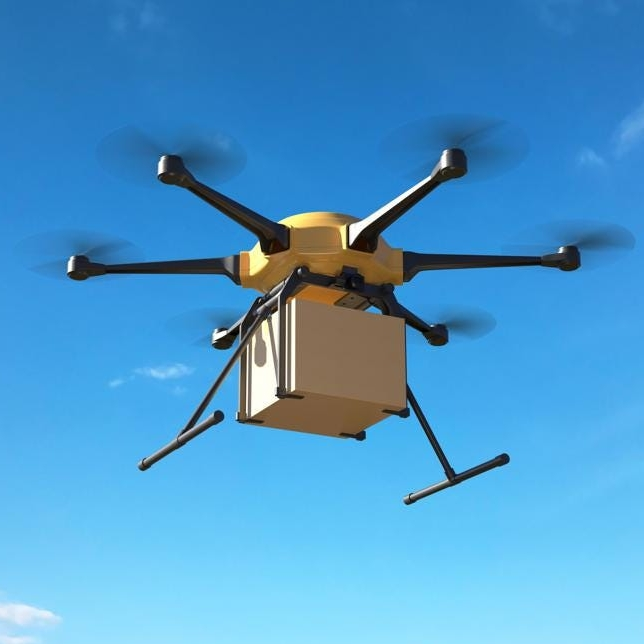
\includegraphics[width=0.9\linewidth]{rigid.jpg}
            \caption{Rigid connection \cite{Wolf2020}}
        \end{subfigure}
        \begin{subfigure}[t]{0.32\textwidth}
            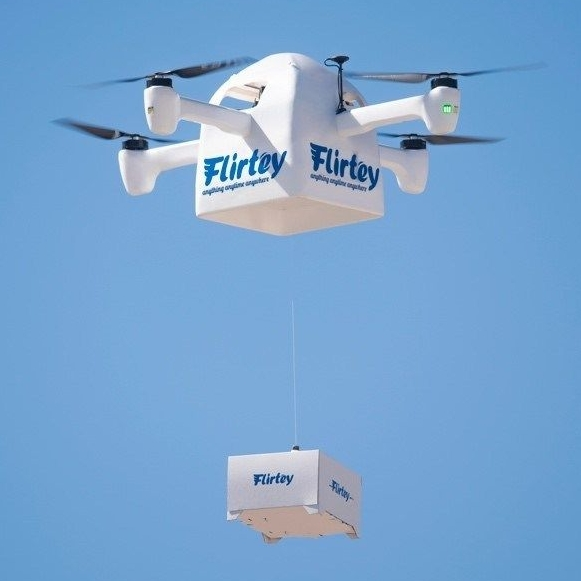
\includegraphics[width=0.9\linewidth]{suspended.jpg}
            \caption{Suspended cable \cite{Flirtey}}
        \end{subfigure}
        \begin{subfigure}[t]{0.32\textwidth}
            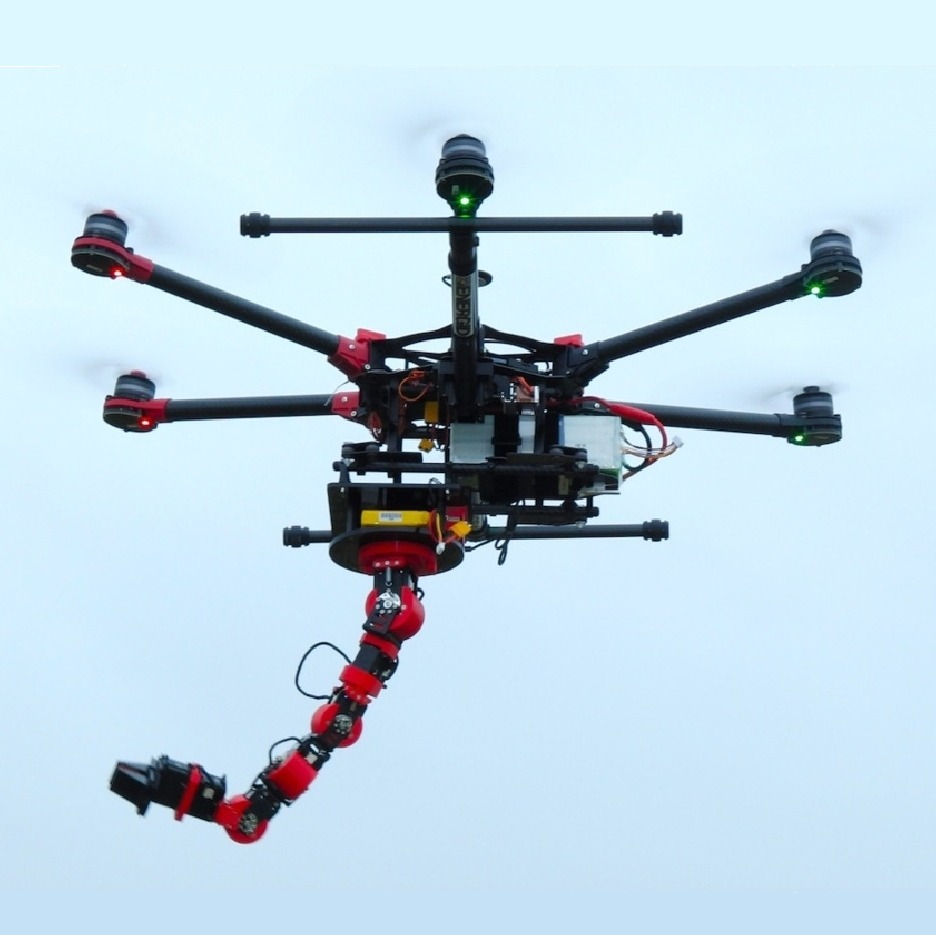
\includegraphics[width=0.9\linewidth]{actuated_payload_blue_bg.jpg}
            \caption{Robotic actuator \cite{Tardella2016}}
        \end{subfigure}
        \caption{Different multirotor payload configurations}
        \label{fig:rigid_suspended_actuated} 
    \end{figure}

    \subsection{Rigid connection payloads}

        \paragraph
        Payloads are often rigidly attached to a multirotor for transportation.
        This configuration is especially popular for commercial package deliveries \cite{San2018}.
        There is minimal relative movement between the multirotor and the rigidly connected payload, hence, the payload only affects the \gls{CoM}, the moment of inertia, and the aerodynamics of the vehicle.
        Often, the weight and size of the payload is unknown prior to flight.
        
        \paragraph
        Different control approaches have been proposed to deal with the altered flight dynamics for this applications, 
        including \gls{ARC} \cite{Min2011} and \gls{MRAC} \cite{Emran2015}.
        These control architectures mostly involve a parameter estimation algorithm to estimate the inertial parameters,
        and an adaptive control law based on the estimated parameters and predetermined dynamical model of the system.

        % \paragraph
        % \citet{Mellinger2011a} proposed an adaptive controller for a multirotor with a rigidly connected payload.
        % Least-squares estimation techniques were applied to estimate the inertial parameters of the payload.
        % A adaptive control law was then applied which uses the estimated parameters in the control law.
        % Experimental results showed acceptable trajectory tracking performance with the adaptive controller.

        \paragraph
        An advantage of rigidly connected payloads is that the flight dynamics is not altered significantly.
        The payload does not add a degree of freedom to the system and only the inertial parameters need to be accounted for.
        However, this configuration limits the shape and size of a potential payload, since
        the payload needs to be compatible with the vehicle gripper.
        The multirotor also needs to land or approach the payload very closely to attach to the load, which may be impractical in many applications.

    \subsection{Suspended payloads}

        \paragraph
        Figure~\ref{fig:real_suspended_payload_example} shows an example of a practical application of a suspended payload used during search and rescue missions.
        The shape and mass of the payload has an effect on the flight dynamics, but the payload is often unknown prior to flight.
        The control system should be able to account for these uncertainties and fly well despite the altered flight dynamics.

        \begin{figure}[htb]
            \centering
            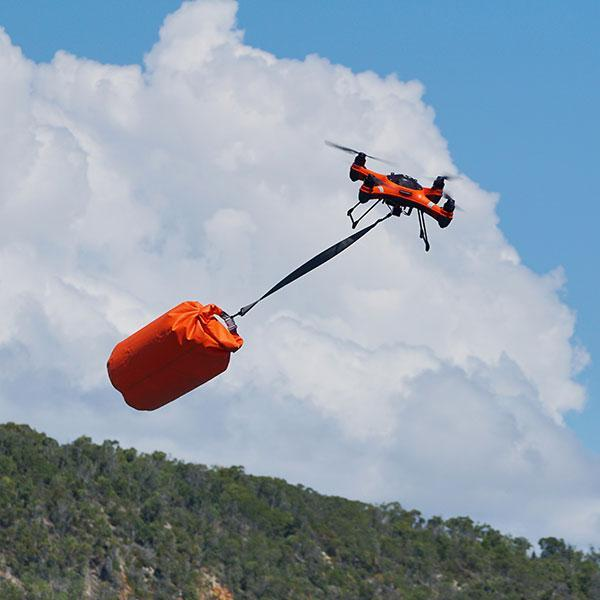
\includegraphics[width=0.45\linewidth]{real_suspended_payload_example.jpg}            
            \caption{A practical suspended payload used for search and rescue missions \cite{CompareCommander2020}}
            \label{fig:real_suspended_payload_example}
        \end{figure}

        \paragraph
        Various suspended payload configurations have been considered in literature.
        The classical suspended payload application involves a small payload suspended below the vehicle with rigid link \cite{Erasmus2020, Slabber2020, Guerrero-Sanchez2017, Klausen2017, Ichikawa2018, DeAngelis2019a}. 
        \citet{Kotaru2017} considered a suspended payload system with an elastic cable modelled as a spring-damper system.
        \citet{Tang2015a} modelled the multirotor-payload system with a hybrid dynamical model to consider aggressive manoeuvres where the cable transitions from taut to slack.
        The transportation of payload loads with flexible cables have also been studied, where the cable is modelled as a set of serially-connected rigid links  \cite{Goodarzi2015, Goodarzi2014, Kotaru2018}. 
        Furthermore, the control of a group of multirotors cooperatively transporting a suspended payload have also been considered in various studies \cite{Lee2015, Sanalitro2020, Klausen2014, Goodarzi2015}.
        
        \paragraph % This paragraph seems out of place and does not flow well
        From numerous examples in literature, it is clear that the control of multirotors with suspended payloads is a popular research topic.
        The suspended payload configuration is very useful in situations where a multirotor cannot land, since the payload can be attached during hover.
        This configuration also has the advantage that a load can have an arbitrary shape or size as long as it has an attachment point for a cable.
        However, the suspended payload increases the degrees of underactuation of the system, which makes the control problem challenging \cite{Kotaru2018}.

        % ?? Fi author cite and [12-15] to rather [12,13,14,15]
\section{Control of multirotors with suspended payloads}

    \paragraph
    A major drawback of transporting a suspended payload is that the payload is free to swing during flight, which effects the dynamics of a multirotor.
    Two main control strategies are applied in literature to stabilise a multirotor with a suspended payload, namely, trajectory generation and active vibration damping.
    Some methods combine the two methods into a single control architecture.
    Trajectory generation methods involve determining multirotor trajectories that result in minimal oscillations or specific payload trajectories.
    Active vibration damping controllers involve feedback controllers that apply a control law to actively counteract the swing of the payload.

    \subsection{Trajectory generation}

        \paragraph
        Trajectory generation methods for suspended payload systems are based on open-loop control techniques.
        The objective of these techniques is to determine a trajectory in which the multirotor motion would induces a specific payload trajectory to reduce oscillations or avoid obstacles.
        Numerous trajectory generation methods have been explored in literature for suspended payload transportation 
        \cite{Tang2015b, Geisert2016, Zeng2019, Xian2020, Starr2005, Palunko2012, Su2019, Palunko2013, Faust2013}. % ?? Maybe remove this long citation?

        \paragraph
        \citet{Zeng2019} and \citet{Tang2015b} applied differential flatness based trajectory planning methods for multirotors in obstacle-filled environments.
        Instead of only considering swing-reduction of the suspended payloads, these studies consider specific payload trajectories to avoid obstacles during aggressive motion.
        \citet{Xian2020} proposed an efficient online trajectory planning method without iterative optimizations.
        The swing-reduction performance of this method was also verified with experimental results.
        
        \paragraph
        Dynamic programming methods have also been implemented to generate swing-free trajectories with suspended payloads \cite{Starr2005, Palunko2012, Su2019}.
        These methods require accurate models of the plant dynamics and are sensitive to the accuracy of these models.
        \gls{RL} methods do not require prior models of the dynamics and have also been applied for swing-free trajectory generation \cite{Palunko2013, Faust2013}.
        \citet{Faust2013} implemented a \gls{RL} method for minimal swing trajectories which provides sufficient criteria to allow the learned policy to be transferred to a variety of different models, starting positions, and trajectories.
        Furthermore, this \gls{RL} trajectory generation method was verified with simulation and experimental results.
        % ?? Maybe continue this and explain more

        % Look for newer literature. ??

        % ?? Maybe add this
        % \paragraph 
        % A drawback of \gls{MPC} and \gls{RL} methods is that they rely on cost functions with tuning weights and linear constraints for obstacle avoidance.
        % \citet{Silveira2020} addressed this problem by implementing a \gls{RRT} algorithm that does not rely on cost functions and constraints for collision-free trajectories with a suspended payload.
        % However, this approach does not provide an optimal solution, but rather finds any collision-free trajectory as a solution. 

        \paragraph
        Input shaping is another open-loop control method applied for minimal swing control that is related to trajectory planning.
        This technique involves modifying a reference signal, usually with a set of timed impulses, to cancel oscillatory modes of the system \cite{Vaughan2008}.
        These techniques were originally designed for transporting suspended payloads using gantry systems \cite{Smith1957, Starr1983}.
        Later, these input shaping techniques were also applied for reduced swing control of 
        helicopters \cite{Bisgaard2008, Potter2011} and 
        multirotors \cite{Homolka2017, Sadr2014b, Fielding2019} that carry suspended payloads.

        \paragraph
        \citet{Ichikawa2018a} compared different input shaping techniques for velocity control of a quadrotor with a suspended payload in simulations.
        The specific input shaping techniques considered were: \gls{ZV}, \gls{NZV}, \gls{EI}, and 2-hump \gls{EI}.
        These methods convolve a baseline input command with precisely timed impulses based on the length of the suspended cable. 
        Simulation results showed that the input shapers significantly decreased the residual payload oscillations compared to a baseline velocity controller.
        It was highlighted that \gls{EI} and 2-hump \gls{EI} were more robust to cable length uncertainty than \gls{ZV} and \gls{NZV}.

        \paragraph
        \citet{Slabber2020} applied a notch filter to reduce payload oscillations for velocity control of a multirotor in simulation.
        \citet{Slabber2020} considered a system with unknown payload parameters.
        The unknown payload mass and cable length were estimated with \gls{RLS} and \gls{FFT} parameter estimators respectively and
        the natural frequency was calculated based on these estimates.
        The notch filter was applied to the velocity setpoint signal to suppress the frequency band containing this natural frequency. 
        \citet{Slabber2020} showed that a wider frequency band could be used to improve robustness against parameter uncertainty.
        It was shown in simulation that the notch filter attenuated the payload oscillations to a near swing free motion even with large parameter estimation errors \cite{Slabber2020}.
    
    \FloatBarrier\subsection{Swing damping controllers}

        % ?? Add pictures

        \paragraph
        Swing damping control is a closed-loop control method where a feedback control law is applied that directly affects the payload states.
        This control method is also referred to as active vibration damping.
        Instead of finding a trajectory that reduces oscillations, these controllers follow a given trajectory as close as possible while trying to reduce payload oscillations.
         
        % ?? Check if all citations refer to correct work. Sometimes copied wrongly

        \paragraph
        \gls{LQR} is a popular optimal control technique and has often been used as a baseline controller to evaluate the performance of other swing damping controllers for multirotors with suspended payloads \cite{Trachte2014, Alothman2018a, Alothman2018b, Slabber2020, Alothman2016, Notter2016}.
        \citet{Erasmus2020article} proposed \gls{LQG} control for swing damping control of a multirotor with suspended cable.
        The payload state remained unmeasured and a \gls{EKF} was implemented for full-state estimation of the multirotor-payload system.
        The \gls{EKF} was combined with an \gls{LQR} full-state feedback controller to produce \gls{LQG} control.
        Simulation results showed good swing damping control with position step inputs despite the unmeasured payload state, external disturbances, sensor noise, and parameter uncertainty.

        \paragraph
        \citet{Slabber2020} implemented a \gls{LQR} controller augmented with a notch filter input shaper for improved swing damping performance.
        The notch filter was applied to the velocity step reference and the 
        \gls{LQR} was then applied with the filtered reference signal for swing-damping control.
        The \gls{LQR} was designed with integral action added to the velocity state to ensure zero steady-state velocity tracking. 
        Furthermore, this work involved estimating the unknown payload state with a vision-based estimator for use in the full-state feedback controller. 
        Simulation results showed that this controller provides good swing damping performance in the presence of external disturbances, sensor noise, and parameter uncertainty. 

        \paragraph
        \gls{MPC} is an optimal control technique related to \gls{LQR} that has also been applied to suspended payload systems.
        % \gls{MPC} solves control optimisation problem over a finite prediction horizon at every control interval based on a separately identifiable plant model \cite{Mayne2000}.
        \citet{Notter2016} implemented an \gls{MPC} for active swing damping control of a quadrotor with a suspended payload.
        A non-linear model of the quadrotor-payload system was linearised and discretised to apply a discrete, linear \gls{MPC} formulation.
        The physical parameters of the quadrotor, cable, and payload were assumed to be exactly known and the controller is tested with only one payload.
        The controller received a position trajectory reference and determined force setpoints to control the vehicle.
        Furthermore, constraints were applied to the heigh, attitude, and control inputs to ensure safe flight manoeuvres. 
        Simulation results showed superior trajectory tracking performance of the \gls{MPC} compared to a baseline \gls{LQR} controller.
        The \gls{MPC} simulation results were also verified with experimental results in an practical indoor environment.

        \paragraph
        \citet{Santos2018} implemented a robust tube-based \gls{MPC} for trajectory tracking and payload stabilisation of a tilt-rotor \gls{UAV} and suspended payload. 
        This approach consists of a pre-stabilising control policy for the nominal system and an additive control policy for mismatch error. 
        The \gls{MPC} was applied as a outer-loop position controller, and a mixed $\mathcal{H}_2 / \mathcal{H}_\infty$ controller was applied for inner-loop attitude control.
        Integral action is applied in the \gls{MPC} to position states to ensure zero steady-state error with external disturbances and modelling errors.
        
        \paragraph
        % A discrete, linear state-space plant model is derived and used in the \gls{MPC}.
        The tube-based \gls{MPC} is designed to be robust against the additive uncertainties from the decoupling, linearization and discretisation modelling errors.
        However, physical parameters of the model are assumed to be exactly known and non-additive parameter uncertainty is not considered.
        Simulation results showed stabilised control of the system is achievable with this control architecture along a square-like trajectory with sharp corners.

        \paragraph
        Other types of controller have also been applied for active swing damping and will be discussed in Section~\ref{sec:review_swing_damping}.
        Active swing damping controllers generally perform better than open-loop, trajectory generation methods for systems with model uncertainties and external disturbances \cite{Liang2021}.
        This is expected, since trajectory generation requires accurate plant models and small modelling uncertainties can significantly alter a trajectory.
        Active swing damping controllers will be focused on in the remainder of this study.

    % ?? Fix Table of literature
% https://docs.google.com/spreadsheets/d/1jw2rWzO23fUF4sSDTCzJE1Sc9mvNLo3NGZaDicredc8/edit#gid=1305340631


\newpage % or \pagebreak

\begin{landscape}
    \begin{tiny}

% \begin{table}[!h]
%     \mytable
%     \caption{Performance of the unconstrained segmental Bayesian model on TIDigits1 over iterations in which the reference set is refined.}
%     \begin{tabularx}{\linewidth}{@{}lCCCCC@{}}
%         \toprule
%         Metric     & 1 & 2 & 3 & 4 & 5 \\
%         \midrule
%         WER (\%)                        & $35.4$ & $23.5$ & $21.5$ & $21.2$ & $22.9$ \\
%         Average cluster purity (\%)       & $86.5$ & $89.7$ & $89.2$ & $88.5$ & $86.6$ \\
%         Word boundary $F$-score (\%)         & $70.6$ & $72.2$ & $71.8$ & $70.9$ & $69.4$ \\
%         Clusters covering 90\% of data   & 20             & 13 & 13 & 13 & 13 \\
%         \bottomrule
%     \end{tabularx}
%     \label{tbl:exemplars}
% \end{table}

\begin{table}[!htbp]
    \renewcommand{\arraystretch}{1.1}
    \centering
    \caption{Summary of literature considered regarding swing damping control of multirotors with suspended payloads}
    \begin{tabularx}{\linewidth}{@{}lllllllllll@{}}
        \toprule
            \textbf{Author}              & \textbf{Year}                   & \textbf{Proposed}          & \textbf{Baseline}      & \textbf{Plant model} & \textbf{Parameter} & \textbf{Unknown} & \textbf{Unmeasured} & \textbf{Different} & \textbf{Practical} & \textbf{Outdoor} \\
        \midrule
            \citet{Muthusamy2021a}       & \citeyear{Muthusamy2021a}       & \gls{BFBEL}                & -                      & none                 & yes                & yes              & yes                 &                    & yes                &                  \\
            \citet{Hua2021}              & \citeyear{Hua2021}              & \gls{RL} (nonlinear)       & \gls{BS}, Energy-based & none                 & yes                & yes              &                     &                    & yes                &                  \\
            \citet{Allahverdy2021}       & \citeyear{Allahverdy2021}       & \gls{BISMC} with \gls{ILC} & -                      & non-linear           & yes                & yes              &                     &                    &                    &                  \\
            \citet{Faust2014}            & \citeyear{Faust2014}            & \gls{RL} (\gls{CAFVI})     & -                      & none                 & yes                & yes              &                     &                    & yes                &                  \\
            \citet{Wang2020}             & \citeyear{Wang2020}             & \gls{ADRC}                 & -                      & linear               & yes                & yes              & yes                 &                    & yes                & yes              \\
            \citet{Taylor2020}           & \citeyear{Taylor2020}           & \gls{H-inf} loop-shaping   & \gls{LQR}              & linear               & yes                &                  &                     & yes                &                    &                  \\
            \citet{Erasmus2020}          & \citeyear{Erasmus2020}          & \gls{MRAC}                 & \gls{LQR}              & linear               & yes                &                  & yes                 & yes                & yes                & yes              \\
            \citet{Slabber2020}          & \citeyear{Slabber2020}          & \gls{LQR}                  &                        & linear               & yes                &                  &                     & yes                &                    &                  \\
            \citet{Dai2014}              & \citeyear{Dai2014}              & \gls{RCAC}                 & -                      & non-linear           & yes                &                  &                     &                    &                    &                  \\
            \citet{Santos2016}           & \citeyear{Santos2016}           & \gls{MPC}                  & -                      & linear               & yes                &                  &                     &                    &                    &                  \\
            \citet{Andrade2016}          & \citeyear{Andrade2016}          & \gls{MPC}                  & \gls{LQR}              & linear               & yes                &                  &                     &                    &                    &                  \\
            \citet{Zurn2016}             & \citeyear{Zurn2016}             & \gls{MPC}                  & -                      & linear               &                    &                  &                     &                    & yes                &                  \\
            \citet{Son2019}              & \citeyear{Son2019}              & \gls{MPC}                  & -                      & linear               &                    &                  &                     &                    & yes                &                  \\
            \citet{Son2018}              & \citeyear{Son2018}              & \gls{MPC}                  & -                      & linear               &                    &                  &                     &                    & yes                &                  \\
            \citet{Son2017}              & \citeyear{Son2017}              & \gls{MPC}                  & -                      & linear               &                    &                  &                     &                    &                    &                  \\
            \citet{Trachte2014}          & \citeyear{Trachte2014}          & \gls{MPC}                  & \gls{LQR}              & non-linear           &                    &                  &                     &                    &                    &                  \\
            \citet{Trachte2015}          & \citeyear{Trachte2015}          & \gls{MPC}                  & \gls{LQR}              & non-linear           &                    &                  &                     &                    &                    &                  \\
            \citet{Liang2021}            & \citeyear{Liang2021}            & Nonlinear                  & \gls{LQR}, \gls{PD}    & non-linear           &                    &                  &                     & yes                & yes                &                  \\
            \citet{Zeng2019a}            & \citeyear{Zeng2019a}            & Geometric                  & -                      & non-linear           &                    &                  &                     &                    &                    &                  \\
            \citet{Yang2018}             & \citeyear{Yang2018}             & \gls{RISE}                 & -                      & non-linear           &                    &                  &                     &                    &                    &                  \\
            \citet{Martinez-Vasquez2020} & \citeyear{Martinez-Vasquez2020} & \gls{SMC}                  & -                      & linear               &                    &                  &                     &                    &                    &                  \\
            \citet{Mosco-Luciano2020}    & \citeyear{Mosco-Luciano2020}    & \gls{BS}                   & -                      & linear               &                    &                  &                     &                    & yes                &                  \\
            \citet{Rigatos2018}          & \citeyear{Rigatos2018}          & \gls{H-inf}                & -                      & linear               &                    &                  &                     &                    &                    &                  \\
            \citet{Alothman2015}         & \citeyear{Alothman2015}         & \gls{LQR}                  & \gls{PD}               & linear               &                    &                  &                     &                    &                    &                  \\
            \citet{Alothman2016}         & \citeyear{Alothman2016}         & \gls{iLQR}                 & \gls{LQR}              & linear               &                    &                  &                     &                    &                    &                  \\
        \bottomrule
    \end{tabularx}
    \label{tbl:lit}
\end{table}

% Add \\ to last line otherwise error.
% Use tabularx
% ?? Remove year column to save space

    \end{tiny}
\end{landscape}



    \FloatBarrier\section{Review of swing damping control studies} \label{sec:review_swing_damping}
    
        \paragraph
        This section will discuss trends in literature regarding the swing damping control of multirotors with suspended payloads.
        Table~\ref{tbl:lit} lists other works in literature involving the active swing damping control of multirotors with suspended payloads.
        Studies that exclusively consider trajectory generation or cooperative transportation of a payload with multiple multirotors are excluded from this table.
        From Table~\ref{tbl:lit}, it is clear that transportation of a suspended payload with a multirotor is a popular and current research topic.
        
        \paragraph
        For each study in Table~\ref{tbl:lit}, the type of proposed controller is listed along with a baseline controller if applicable.
        Baseline controllers are well known techniques applied to a considered problem to compare the performance of a proposed technique to a reference performance.
        Other studies compare different variations of the proposed controller to highlight the effect of design decisions, but these comparisons are not considered as baseline comparisons. 
        Many studies in Table~\ref{tbl:lit} do not consider a baseline controller, which makes it difficult to evaluate the performance of the proposed technique objectively.
        These studies can conclude that a proposed techniques solves the considered problem, but it is not conclusive whether the technique improves on the performance of known controllers.
        However, from Table~\ref{tbl:lit} it is clear that \gls{LQR} is a popular baseline controller for active swing damping techniques and especially for optimal control techniques.

        \paragraph
        From the studies considered in Table~\ref{tbl:lit}, it also appears that \gls{MPC} is a popular technique for the considered control objective.
        Historically, \gls{MPC} was designed for slow moving processes in the chemical industry because the computational intensity of this method limited the controller frequency on the available hardware \cite{Lee2011}.
        However, due to improvements in the speed of computational hardware, \gls{MPC} has become a viable controller for faster systems.
        Various \gls{MPC} implementations were successfully applied in experimental flight tests which shows that \gls{MPC} is suitable for practical multirotor implementations \cite{Zurn2016, Son2019, Son2018}
        
        \paragraph
        It is also noted that most proposed controllers, including \gls{MPC} implementation, are based on a linearised plant model of the non-linear multirotor-payload dynamics.
        This shows that a linearised plant model can provide a sufficient representation of the suspended payload dynamics for effective swing damping control.
        % In some studies, seperate controllers are applied to different parts of the control problem where the plant models considered by some controllers are non-linear, and others are linear \cite{Martinez-Vasquez2020}.
        % In Table~\ref{tbl:lit}, the \emph{Plant model} column considers the specific model that includes the suspended payload dynamics.
        Non-linear \gls{MPC} implementations which depend on a non-linear plant model have also been studied for the quadrotor with a suspended payload \cite{Trachte2014, Trachte2015}.
        However, the non-linear \gls{MPC} results were not compared to linear \gls{MPC} results, therefore the studies do not conclusively justify the need for a non-linear plant model.
        Non-linear \gls{MPC} is more computationally intensive than linear \gls{MPC}, which makes it more challenging to implement in real-time for practical flights.
        None of the studies considered in Table~\ref{tbl:lit} that were implemented on practical systems used non-linear plant models.
        However, some practical implementation apply controllers which do not depend on a plant model and show promising results \cite{Muthusamy2021, Hua2021, Faust2014}.

        \paragraph
        Note from Table~\ref{tbl:lit}, that many studies only consider the proposed controllers in simulation and do not include practical data.
        Practical data may include sensor noise, modelling uncertainties, external disturbances, and other computational hardware effects like latency that are often not considered in simulation.
        Unlike simulation results, experimental results clearly show that a proposed method is suitable for real-life applications.
        These results also show that the proposed algorithms can run in real-time on the available hardware, which is often a challenge for complex techniques.
        
        \begin{figure}[ht]
            \centering
            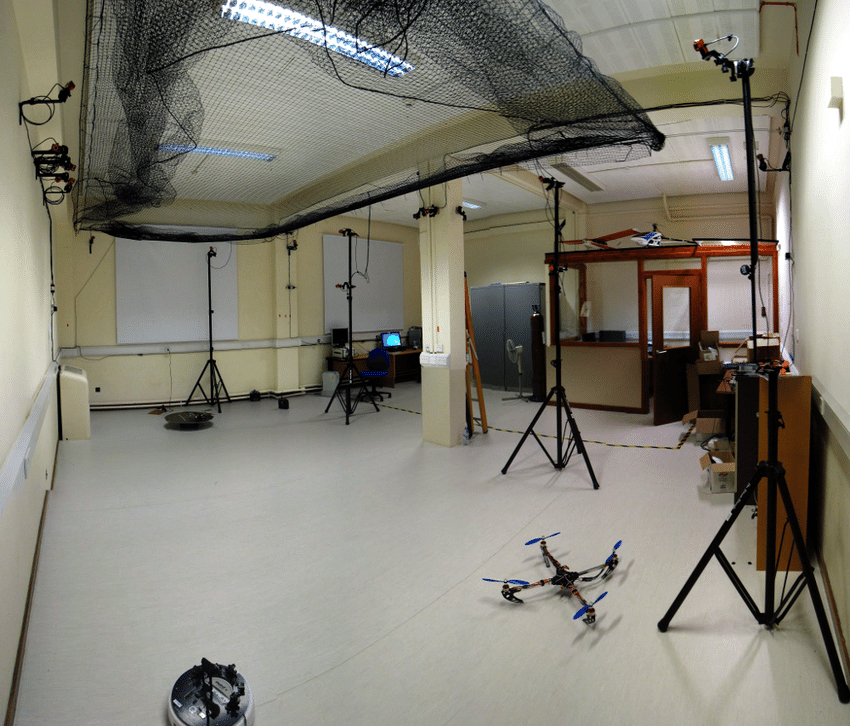
\includegraphics[width=0.6\linewidth]{lit_study/fig/motion_capture}
            \caption{Optitrack motion capture system for multirotor experiments \cite{Ireland2014}}
            \label{fig:motion_capture}
        \end{figure}        

        \paragraph
        It is also noted that few studies in the literature consider outdoor flights.
        Most studies only consider practical flights performed in controlled indoor environments.
        Figure~\ref{fig:motion_capture} shows an indoor motion capture setup used for multirotor experiments.
        In these experiments, motion capture systems like Vicon \cite{Muthusamy2021, Hua2021, Faust2014, Zurn2016, Son2019, Son2018}, Qualisys \cite{Liang2021} or Optitrack \cite{Mosco-Luciano2020} provide high accuracy state feedback data at rates of \SI{100}{\hertz} or more.
        This type of setup is often impractical for real-life multirotor applications.
        
        \paragraph
        Outdoor payload transportation is dependant on state feedback from inaccurate sensors like \gls{GPS} and potentiometers, which greatly increase the difficulty of the control problem.
        The multirotor-payload system may also be exposed to uncontrolled wind disturbances which further complicates the control problem.
        Figure~\ref{fig:outdoor_setup} shows a multirotor in an outdoor practical experiment with a suspended payload \cite{Wang2020}.

        \begin{figure}[ht]
            \centering
            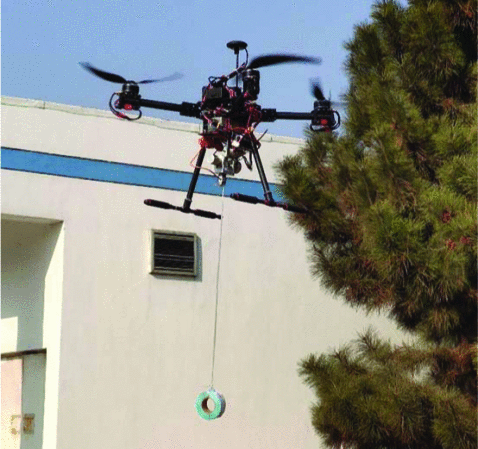
\includegraphics[width=0.6\linewidth]{lit_study/fig/outdoor_setup.png}
            \caption{Multirotor and suspended payload for outdoor experiments \cite{Wang2020}}
            \label{fig:outdoor_setup}
        \end{figure}  
        
        \paragraph
        As observed by \citet{Hua2021}, most reported controllers in literature are designed based on accurate plant models without considering dynamical uncertainties in the studies.
        This is also evident from the literature considered in Table~\ref{tbl:lit}.
        The \emph{Parameter uncertainty} column identifies studies that account for parameter uncertainty in the considered plant model.
        Many controllers account for uncertainty in the parameter values of the plant model.
        These controllers either apply robust techniques \cite{Taylor2020} to ensure stability despite the parameter uncertainty, or adaptive techniques \cite{Dai2014} to change the control law to result in improved control with the resultant dynamics.
        Other controllers combine robust and adaptive techniques into a single control architecture \cite{Erasmus2020, Slabber2020}.
        
        \paragraph
        It is interesting to note that very few of these studies test the proposed controllers on more than one payload.
        The \emph{Different payloads} column identifies studies that consider more than one payload.
        Other studies designed controllers to account parameter uncertainty, but only tested the tuned controller on a single payload case.
        This does not conclusively demonstrate the adaptability or robustness of a controller, 
        since the payload could be cherry-picked or the controller could be specifically tuned for one payload.
        It is therefore noted that it is valuable to demonstrate a controller on multiple payload cases.

        \paragraph
        In Table~\ref{tbl:lit}, the \emph{Unknown dynamics} column identifies studies that account for unknown dynamics of a multirotor with a suspended payload.
        This does not include uncertainty due to modelling errors as a result of a priori linearisation and discretisation.
        These studies make minimal assumptions regarding the dynamics of the payload and propose stabilising controllers that are effective despite the unknown dynamics.
        This approach is useful for complicated working conditions with model uncertainties \cite{Hua2021}.
        It is also interesting to note by the publication dates that most of these studies are quite recent.
        This appears to be a promising research area that has been considered in only a few different studies.

\section{Multirotor and suspended payload systems with unknown dynamics}

    \paragraph
    Only a few studies have been identified that consider stabilised control of a multirotor and suspended payload without prior knowledge of the payload dynamics \cite{Muthusamy2021, Allahverdy2021, Faust2014, Wang2020}.
    Some methods are not based on a plant model and learn a stabilising control law without knowledge of the system dynamics \cite{Muthusamy2021, Faust2014}.
    Other strategies control the multirotor with an model based method and consider the effect of the suspended payload as an external disturbance \cite{Wang2020, Allahverdy2021}

    \begin{figure}[ht]
        \centering
        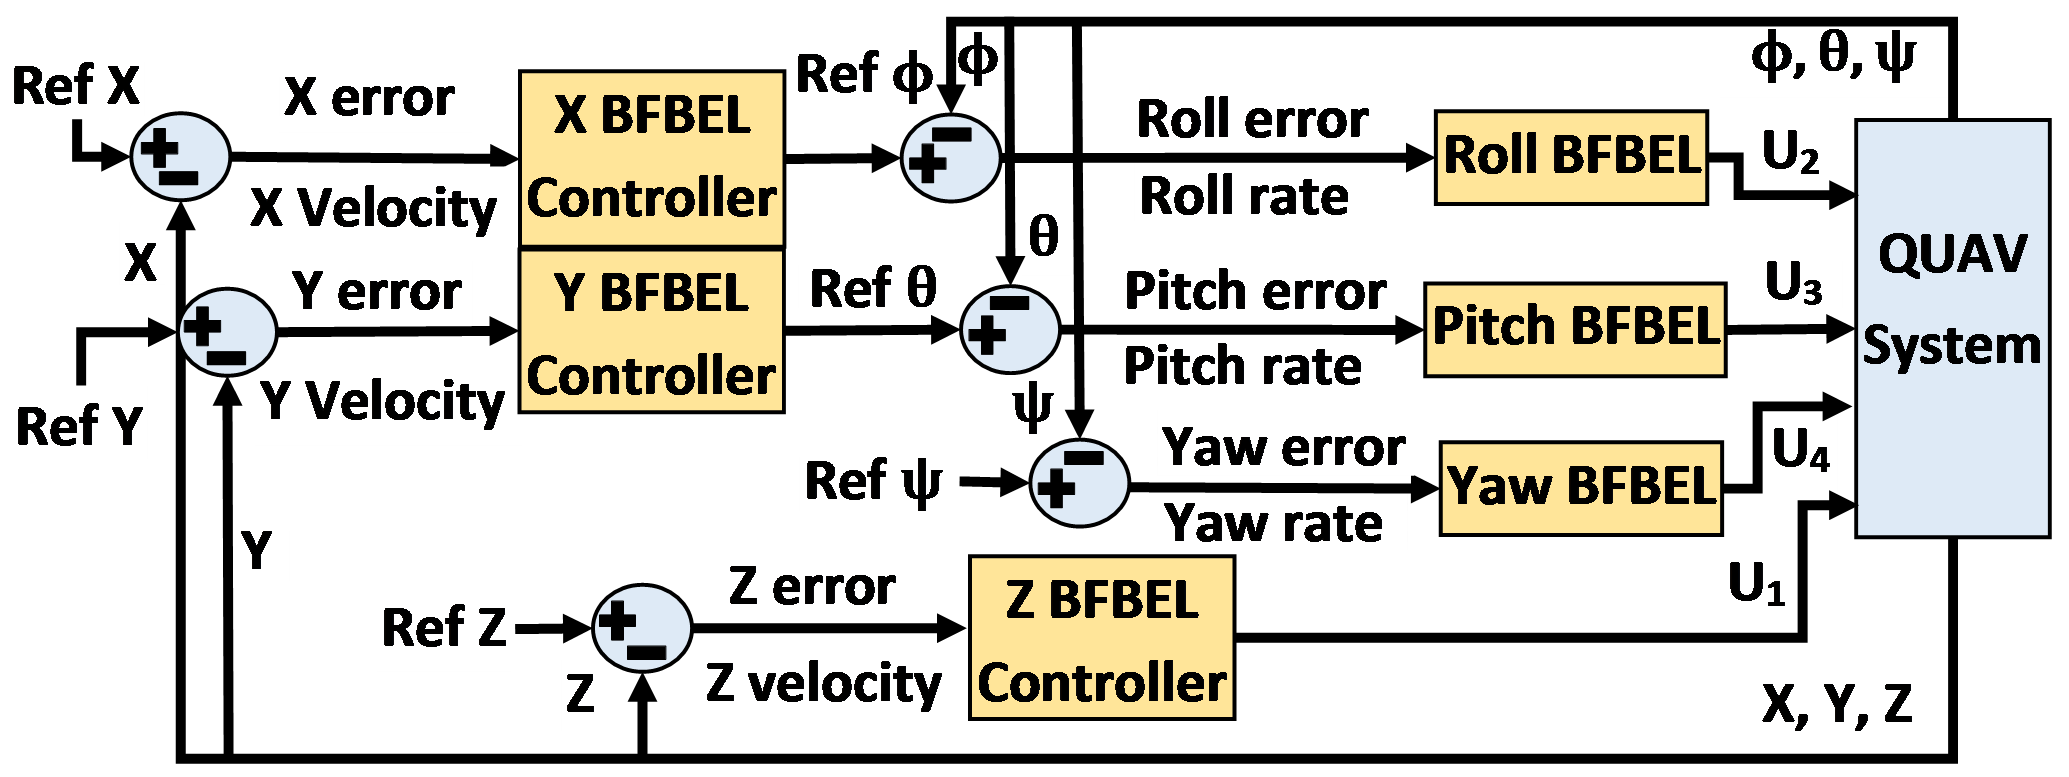
\includegraphics[width=0.8\linewidth]{lit_study/fig/BFBEL.png}
        \caption{Controller structure proposed by \citet{Muthusamy2021}}
        \label{fig:BFBEL}
    \end{figure} 

    \paragraph
    \citet{Muthusamy2021} proposed a \gls{BFBEL} controller which incorporates fuzzy inference, neural networks and the \gls{BBEL} algorithm.
    A separate \gls{BFBEL} feedback controller is applied to each degree of freedom of the \gls{6DOF} multirotor system, as shown in Figure~\ref{fig:BFBEL}.
    The payload state remains unmeasured and the objective of the controller is to stabilise the multirotor system and provide accurate position tracking without knowledge of the multirotor-payload dynamics.
    Experimental results demonstrate the rapid adaptation capability and the trajectory tracking performance of the proposed \gls{BFBEL} controller.
    Without prior knowledge of the system, the controllers weights are autonomously tuned within \SI{30}{\second} of flight time to provide stable trajectory tracking of the multirotor.
    The payload state is not explicitly measured or damped, causing residual oscillations in the position data of the multirotor.

    \paragraph
    A double \gls{ADRC} was proposed by \citet{Wang2020} for the control of a multirotor with an unknown suspended payload.
    A second-order transfer function model of a practical multirotor without a load was determined with a frequency sweep excitation method of each control channel.
    The effect of the suspended load was considered as an external disturbance and \glspl{ESO} were applied in the position and attitude loops to estimate the disturbance.
    An \gls{ADRC} in the position and attitude loop could then actively reject the disturbance caused by the payload to stabilise the system without prior knowledge of the payload dynamics.
    Experimental results showed that the proposed controller stabilised the suspended payload to within a tolerable swing angle faster than a \gls{PID} controller, even though the payload state was unmeasured.
    It was was shown that trajectory tracking was significantly improved.
    It should be noted that this technique did not show significant swing damping performance but rather showed that the controller was robust against the effect of the swinging payload.

    \paragraph
    These methods appear to provide stabilised control of the multirotor despite the effect of an unknown swinging payload, but do not provide optimised control of the entire multirotor-payload system.
    These effects focus on counteracting the swinging payload disturbance as it happens and do not directly learn how to control the unknown payload.
    System identification methods can determine a model of unknown dynamics and a controller can be designed based on the identified plant model for improved control of the entire dynamical system.
    Control architectures involving data-driven model identification and resultant model based controller have been proposed for multirotors \cite{Tran2021, Wang2020},
    however we were not able to find similar studies in the literature relating to model identification and control of a multirotor system which includes an unknown suspended payload.
    
    % \paragraph
    % Non-linear, data-driven techniques like \gls{SINDy} have been proposed as a model identification method with \gls{MPC} to control a fixed wing \gls{UAV} with unknown dynamics \cite{Kaiser2018b}.
    % However, \gls{SINDy} has been shown to be extremely sensitive to noise and rational non-linearities \cite{Kaheman2020c} which are present in the dynamical equations describing a multirotor with a suspended payload.
    % Algorithms have been proposed to improve robustness against rational non-linearities \cite{Mangan2016b, Kaheman2020c}.
    % However, these methods are still inherently sensitive to rational non-linearities which are form a significant part of the strongly coupled multirotor and suspended payload dynamics. 

    % \paragraph
    % Related linear data-driven techniques such as DMDc ... 

\section{Summary} 
        
    \paragraph
    This chapter reviewed a range of different control solutions for a multirotor with suspended payload system.
    A few observations were made regarding the literature on this subject, including the following:
    \begin{enumerate}
        \item Most studied controllers are based on accurate models of the system dynamics.
        \item Swing damping methods perform better than trajectory generation methods when considering model uncertainty.
        \item Some studies consider parameter uncertainty, but few studies consider unknown system dynamics.
        \item Few studies that account for parameter uncertainty are demonstrated with different payload parameters.
        \item Methods that consider unknown system dynamics usually consider the suspended payload as an unknown disturbance and do not attempt to actively control the payload.
        \item No studies have been found in the literature that consider data-driven system identification of multirotors with suspended payloads.
    \end{enumerate}

    \paragraph
    The focus of this thesis will involve the stabilised control of a multirotor with a unknown suspended payload.
    The model uncertainty will not only include parameter uncertainty, but the dynamics of the suspended payload system will be considered unknown prior to flight.
    Furthermore, the proposed controller will be based on a estimated model of the multirotor-payload dynamics and it will be tested on different payloads.

}


